\section{Licencias}
\frame
{
	\frametitle{Que son las licencias?}
	\begin{itemize}
	\item Una \textbf{Licencia de software} (en ingles software license) es la autorizacion o permiso concedida por el titular del derecho de autor, en cualquier forma contractual, al usuario de un programa informatico, para utilizar este en una forma determinada y de conformidad con unas condiciones convenidas.La licencia, que puede ser gratuita u onerosa, precisa los derechos (de uso, modificaci� y/o redistribucion) concedidos a la persona autorizada y sus limites. Ademas, puede se�lar el plazo de duraci�, el territorio de aplicacion y todas las demas cl�sulas que el titular del derecho de autor establezca.
	\end{itemize}
}


\subsection{Tipos Licencias}
\frame
{
	\frametitle{Tipos}
	\begin{itemize}
	\item \textbf{Segun derechos que cada autor otorga}
		\begin{itemize}
		\item \textbf{Licencia de software libre sin protecci� heredada}
			\begin{itemize}
			\item Se puede crear una obra derivada sin que esta tenga obligaci� de protecci� alguna. Muchas licencias pertenecen a esta clase, entre otras:
			\item BSD License.
			\item MIT License.
			\end{itemize}
		
		\item \textbf{Licencia de software libre con protecci� heredada}
			\begin{itemize}
			\item Licencia irrenunciable, obra derivada protegida.
			\item GNU General Public License v.2.0.
			\item Mozilla Public License.
			\end{itemize}
		\item \textbf{Licencia de software NO libre}
			\begin{itemize}
			\item Se protege contra uso, copia y/o redistribuci�.
			\item MS-EULA.
			\end{itemize}
			
		\end{itemize}

		
	\item \textbf{Segun su destinatario}
		\begin{itemize}
		\item Licencia de Usuario FinalEn ingl� EULA o end user license agreement, es una licencia en que se permite s�o el uso del mismo.
		\end{itemize}
	\end{itemize}
}
\subsection{Clasificacion}
\frame
{
        \frametitle{Clasificacion}
        \begin{itemize}
     	\item \textbf{Software libre}
		\begin{itemize}
		\item Puede ser usado, copiado, estudiado, modificado y redistribuido libremente.
		\item Disponible gratuitamente en Internet
		\item Puede ser vendido comercialmente.
		\end{itemize}
	\item \textbf{Software privativo}
		\begin{itemize}
		\item  No es libre ni semilibre. 
		\item Su uso, redistribuci� o modificaci� est�prohibida, o requiere autorizacion.
		\end{itemize}
	\item \textbf{Freeware.}
		\begin{itemize}
		\item  No tiene una definici� clara aceptada
		\item Permiten la redistribuci� pero no la modificaci�. Codigo fuente no est�disponible
		\item Estos paquetes no son software libre.
		\end{itemize}
	\item \textbf{Shareware.}
		\begin{itemize}
		\item  Viene con autorizaci� para la gente de redistribuir copias
		\item Quien contine haciendo uso de una copia deber�pagar un cargo por licencia.
		\end{itemize}
	\item \textbf{Software Comercial.}
		\begin{itemize}
		\item  Desarrollado por una entidad que tiene la intenci� de hacer dinero del uso del software. 
		\item ``Comercial'' y ``privativo'' no son la misma cosa!.
		\end{itemize}
        \end{itemize}
}
\subsection{Esquema}
\frame
{
	\frametitle{Esquema}
	\begin{center}
	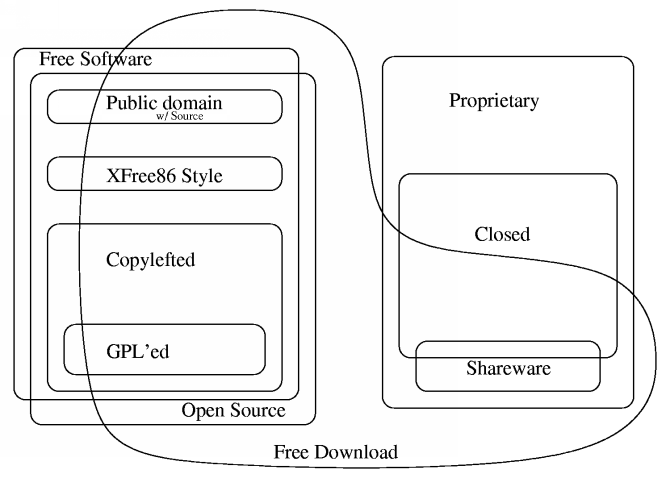
\includegraphics[width=200pt,height=170pt]{category.png}
	\end{center}

}
\subsection{Tres ejemplos concretos}
\frame
{
	\frametitle{Tres ejemplos concretos}
	\begin{itemize}
	\item MS-EULA (End User Licence Agreement
	\item Licencia GPL
	\item Licencia BSD
	\end{itemize}
}
\subsection{MS-EULA (End User Licence Agreement}
\frame
{
	\frametitle{MS-EULA (End User Licence Agreement}
	\begin{itemize}
	\item Se prohibe la copia
	\item El software solo puede ser empleado en un nico ordenador con un m�imo de 2 procesadores
	\item No puede ser empleado como webserver o fileserver.
	\item Puede dejar de funcionar si se efectan cambios en el hardware.
	\item Las actualizaciones del sistema pueden modificar la EULA.
	\item Solo puede ser transferida una vez a otro usuario.
	\item Limita la ingenier� inversa.
	\item S�podr�en cualquier momento recoger informaci� del sistema y su uso, la cual podr�suministrar dicha informaci� a terceros.
	\item La garant� tan solo cubre los primeros 90 d�s.
	\item Actualizaciones y parches sin garant�.
	\end{itemize}
}

\subsection{Licencia GPL}
\frame
{	
	\frametitle{GPL}
	\begin{itemize}
	\item Permite la copia, modificaci� y redistribuci� del software.
	\item Garant� de los derechos del ciudadano a la copia, modificaci� y redistribuci� del software.
	\item No ofrece garant�s sobre el producto.
	\item Puede ser vendido y se puede cobrar por los servicios sobre el software.
	\item Cualquier patente sobre el mismo debe ser licenciada para el beneficio de todos.
	\item Debe incluir el c�igo fuente.
	% Si todos los autores estan de acuerdo, pueden cambiar la licencia
% 	\item \textbf{Desventajas}
% 		\begin{itemize}
% 		\item GPL se dise� para que el c�igo siempre fuese libre, incluso con independencia de la voluntad de sus autores.
% 		\end{itemize}
	\end{itemize}
}
\subsection{Licencia BSD}
\frame	
{
	\frametitle{BSD}
        \begin{itemize}
        \item Software Libre
        \item Cumple con las tres libertades
        \item No es copyleft como la GPL.
        \item Es posible cambiar la licencia.
        \item FreeBSD y el NetBSD.                                                                  
	\item Con los programas BSD, usted est�autorizado a copiarlos y distribuirlos libremente a cuantos quiera y lo podr�hacer por dinero o regal�dolos
        \item \textbf{Desventajas}
		\begin{itemize}
		\item La posibilidad de desarrollar software propietario a partir de un programa BSD.
		\end{itemize}
	\end{itemize}
	
}
